

\tikzset{every picture/.style={line width=0.75pt}} %set default line width to 0.75pt        

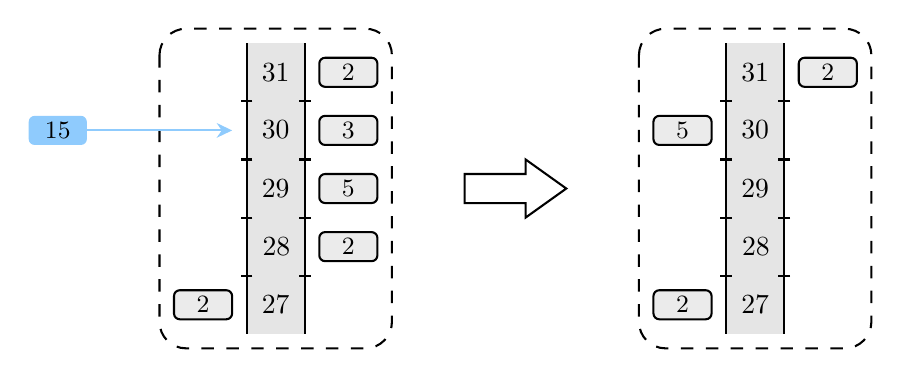
\begin{tikzpicture}[x=0.75pt,y=0.75pt,yscale=-0.7,xscale=0.7]
%uncomment if require: \path (0,300); %set diagram left start at 0, and has height of 300


%Shape: Rectangle [id:dp8412452715917856] 
\draw  [draw opacity=0][fill={rgb, 255:red, 0; green, 0; blue, 0 }  ,fill opacity=0.1 ] (190,50) -- (230,50) -- (230,250) -- (190,250) -- cycle ;
%Rounded Rect [id:dp007986415015731718] 
\draw  [fill={rgb, 255:red, 235; green, 235; blue, 235 }  ,fill opacity=1 ][line width=0.75]  (240,144) .. controls (240,141.79) and (241.79,140) .. (244,140) -- (276,140) .. controls (278.21,140) and (280,141.79) .. (280,144) -- (280,156) .. controls (280,158.21) and (278.21,160) .. (276,160) -- (244,160) .. controls (241.79,160) and (240,158.21) .. (240,156) -- cycle ;
%Straight Lines [id:da2293722746628727] 
\draw    (190,50) -- (190,250) (194,90) -- (186,90)(194,130) -- (186,130)(194,170) -- (186,170)(194,210) -- (186,210) ;
%Straight Lines [id:da3120213615797991] 
\draw    (230,50) -- (230,250) (234,90) -- (226,90)(234,130) -- (226,130)(234,170) -- (226,170)(234,210) -- (226,210) ;
%Rounded Rect [id:dp10621428282249978] 
\draw  [fill={rgb, 255:red, 235; green, 235; blue, 235 }  ,fill opacity=1 ][line width=0.75]  (240,104) .. controls (240,101.79) and (241.79,100) .. (244,100) -- (276,100) .. controls (278.21,100) and (280,101.79) .. (280,104) -- (280,116) .. controls (280,118.21) and (278.21,120) .. (276,120) -- (244,120) .. controls (241.79,120) and (240,118.21) .. (240,116) -- cycle ;
%Rounded Rect [id:dp03800501182586913] 
\draw  [fill={rgb, 255:red, 235; green, 235; blue, 235 }  ,fill opacity=1 ][line width=0.75]  (140,224) .. controls (140,221.79) and (141.79,220) .. (144,220) -- (176,220) .. controls (178.21,220) and (180,221.79) .. (180,224) -- (180,236) .. controls (180,238.21) and (178.21,240) .. (176,240) -- (144,240) .. controls (141.79,240) and (140,238.21) .. (140,236) -- cycle ;
%Rounded Rect [id:dp3338924127776648] 
\draw  [dash pattern={on 4.5pt off 4.5pt}] (130,58.3) .. controls (130,48.19) and (138.19,40) .. (148.3,40) -- (271.7,40) .. controls (281.81,40) and (290,48.19) .. (290,58.3) -- (290,241.7) .. controls (290,251.81) and (281.81,260) .. (271.7,260) -- (148.3,260) .. controls (138.19,260) and (130,251.81) .. (130,241.7) -- cycle ;
%Rounded Rect [id:dp38799186795833285] 
\draw  [fill={rgb, 255:red, 235; green, 235; blue, 235 }  ,fill opacity=1 ][line width=0.75]  (240,64) .. controls (240,61.79) and (241.79,60) .. (244,60) -- (276,60) .. controls (278.21,60) and (280,61.79) .. (280,64) -- (280,76) .. controls (280,78.21) and (278.21,80) .. (276,80) -- (244,80) .. controls (241.79,80) and (240,78.21) .. (240,76) -- cycle ;
%Rounded Rect [id:dp932038680993432] 
\draw  [draw opacity=0][fill={rgb, 255:red, 143; green, 203; blue, 253 }  ,fill opacity=1 ][dash pattern={on 4.5pt off 4.5pt}][line width=0.75]  (40,104) .. controls (40,101.79) and (41.79,100) .. (44,100) -- (76,100) .. controls (78.21,100) and (80,101.79) .. (80,104) -- (80,116) .. controls (80,118.21) and (78.21,120) .. (76,120) -- (44,120) .. controls (41.79,120) and (40,118.21) .. (40,116) -- cycle ;
%Straight Lines [id:da1966192901653835] 
\draw [color={rgb, 255:red, 143; green, 203; blue, 253 }  ,draw opacity=1 ]   (80,110) -- (177,110) ;
\draw [shift={(180,110)}, rotate = 180] [fill={rgb, 255:red, 143; green, 203; blue, 253 }  ,fill opacity=1 ][line width=0.08]  [draw opacity=0] (10.72,-5.15) -- (0,0) -- (10.72,5.15) -- (7.12,0) -- cycle    ;
%Shape: Rectangle [id:dp20325610013103357] 
\draw  [draw opacity=0][fill={rgb, 255:red, 0; green, 0; blue, 0 }  ,fill opacity=0.1 ] (520,50) -- (560,50) -- (560,250) -- (520,250) -- cycle ;
%Rounded Rect [id:dp24083299793098112] 
\draw  [fill={rgb, 255:red, 235; green, 235; blue, 235 }  ,fill opacity=1 ][line width=0.75]  (470,104) .. controls (470,101.79) and (471.79,100) .. (474,100) -- (506,100) .. controls (508.21,100) and (510,101.79) .. (510,104) -- (510,116) .. controls (510,118.21) and (508.21,120) .. (506,120) -- (474,120) .. controls (471.79,120) and (470,118.21) .. (470,116) -- cycle ;
%Straight Lines [id:da7915001823532407] 
\draw    (520,50) -- (520,250) (524,90) -- (516,90)(524,130) -- (516,130)(524,170) -- (516,170)(524,210) -- (516,210) ;
%Straight Lines [id:da9500452904072452] 
\draw    (560,50) -- (560,250) (564,90) -- (556,90)(564,130) -- (556,130)(564,170) -- (556,170)(564,210) -- (556,210) ;
%Rounded Rect [id:dp31551226522886167] 
\draw  [fill={rgb, 255:red, 235; green, 235; blue, 235 }  ,fill opacity=1 ][line width=0.75]  (470,224) .. controls (470,221.79) and (471.79,220) .. (474,220) -- (506,220) .. controls (508.21,220) and (510,221.79) .. (510,224) -- (510,236) .. controls (510,238.21) and (508.21,240) .. (506,240) -- (474,240) .. controls (471.79,240) and (470,238.21) .. (470,236) -- cycle ;
%Rounded Rect [id:dp14842743068542508] 
\draw  [dash pattern={on 4.5pt off 4.5pt}] (460,58.3) .. controls (460,48.19) and (468.19,40) .. (478.3,40) -- (601.7,40) .. controls (611.81,40) and (620,48.19) .. (620,58.3) -- (620,241.7) .. controls (620,251.81) and (611.81,260) .. (601.7,260) -- (478.3,260) .. controls (468.19,260) and (460,251.81) .. (460,241.7) -- cycle ;
%Rounded Rect [id:dp13336948832097884] 
\draw  [fill={rgb, 255:red, 235; green, 235; blue, 235 }  ,fill opacity=1 ][line width=0.75]  (570,64) .. controls (570,61.79) and (571.79,60) .. (574,60) -- (606,60) .. controls (608.21,60) and (610,61.79) .. (610,64) -- (610,76) .. controls (610,78.21) and (608.21,80) .. (606,80) -- (574,80) .. controls (571.79,80) and (570,78.21) .. (570,76) -- cycle ;
%Rounded Rect [id:dp3708973876475854] 
\draw  [fill={rgb, 255:red, 235; green, 235; blue, 235 }  ,fill opacity=1 ][line width=0.75]  (240,184) .. controls (240,181.79) and (241.79,180) .. (244,180) -- (276,180) .. controls (278.21,180) and (280,181.79) .. (280,184) -- (280,196) .. controls (280,198.21) and (278.21,200) .. (276,200) -- (244,200) .. controls (241.79,200) and (240,198.21) .. (240,196) -- cycle ;
%Right Arrow [id:dp26035875111685947] 
\draw   (340,140) -- (382,140) -- (382,130) -- (410,150) -- (382,170) -- (382,160) -- (340,160) -- cycle ;

% Text Node
\draw (210,70) node    {$31$};
% Text Node
\draw (210,109.5) node    {$30$};
% Text Node
\draw (260,150) node  [font=\small]  {$5$};
% Text Node
\draw (210,150) node    {$29$};
% Text Node
\draw (210.5,190) node    {$28$};
% Text Node
\draw (210,230) node    {$27$};
% Text Node
\draw (260,110) node  [font=\small]  {$3$};
% Text Node
\draw (160,230) node  [font=\small]  {$2$};
% Text Node
\draw (260,70) node  [font=\small]  {$2$};
% Text Node
\draw (60,110) node  [font=\small]  {$15$};
% Text Node
\draw (540,70) node    {$31$};
% Text Node
\draw (540,109.5) node    {$30$};
% Text Node
\draw (490,110) node  [font=\small]  {$5$};
% Text Node
\draw (540,150) node    {$29$};
% Text Node
\draw (540.5,190) node    {$28$};
% Text Node
\draw (540,230) node    {$27$};
% Text Node
\draw (490,230) node  [font=\small]  {$2$};
% Text Node
\draw (590,70) node  [font=\small]  {$2$};
% Text Node
\draw (260,190) node  [font=\small]  {$2$};


\end{tikzpicture}
